\documentclass[12pt]{article}


\usepackage{amsfonts,amssymb,latexsym}
\usepackage{amsthm}
\usepackage[margin=1in]{geometry}
\usepackage{graphicx}
\usepackage{amsmath}
\usepackage[font=footnotesize,labelfont=bf]{caption}
\usepackage{subfig}
\usepackage{placeins}
\usepackage{tikz}
\usetikzlibrary{calc,intersections}
\usepackage{bbm}

\newcommand{\N}{\mathbb{N}}
\newcommand{\Z}{\mathbb{Z}}
\newcommand{\Q}{\mathbb{Q}}
\newcommand{\R}{\mathbb{R}}
\newcommand{\C}{\mathbb{C}}
\newcommand{\A}{\mathbb{A}}
\newcommand{\V}{\mathcal{V}}
\newcommand{\I}{\mathcal{I}}
\renewcommand{\P}{\mathbb{P}}
\newcommand{\G}{\mathbb{G}}
\newcommand{\F}{\mathbb{F}}
\newcommand{\B}{\mathbb{B}}
\newcommand{\T}{\mathbb{T}}
\newcommand{\M}{\frak{M}}
\newcommand{\D}{\mathcal{D}}
\renewcommand{\b}{\frak{b}}
\newcommand{\E}{\mathbb{E}}

%   TOPOLOGY   %
%\newcommand{\T}{\mathcal{T}}
%\newcommand{\B}{\mathcal{B}}
%\newcommand{\C}{\mathcal{C}} % do not use with \C for complex numbers above
%\newcommand{\Aball}{\accentset{\circ}{A}}
%\newcommand{\Bball}{\accentset{\circ}{B}}
%\newcommand{\Int}{\text{Int}}
%\newcommand{\Cl}{\text{Cl}}
\newcommand{\Map}{\ensuremath{\operatorname{Map}}}

%   ALGEBRA   %
\newcommand{\diag}{\ensuremath{\operatorname{diag}}}
\newcommand{\Span}{\ensuremath{\operatorname{Span}}}
\newcommand{\codim}{\ensuremath{\operatorname{codim}}}
\newcommand{\Spec}{\ensuremath{\operatorname{Spec}}}
\newcommand{\rad}{\ensuremath{\operatorname{rad}}}
\newcommand{\norm}{\mathrel{\lhd}}
\newcommand{\im}{\ensuremath{\operatorname{im}}}
\newcommand{\coker}{\ensuremath{\operatorname{coker}}}
\newcommand{\rank}{\ensuremath{\operatorname{rank}}}
\renewcommand{\char}{\ensuremath{\operatorname{char}}}
\newcommand{\Aut}{\ensuremath{\operatorname{Aut}}}
\newcommand{\la}{\langle}
\newcommand{\ra}{\rangle}
\newcommand{\orb}{\mathcal{O}}
\newcommand{\obj}{\ensuremath{\operatorname{obj}}}
\newcommand*\cat[1]{{\tt #1}}
\newcommand{\End}{\ensuremath{\operatorname{End}}}
\newcommand{\Hom}{\ensuremath{\operatorname{Hom}}}
\newcommand{\Ext}{\ensuremath{\operatorname{Ext}}}
\newcommand{\Tor}{\ensuremath{\operatorname{Tor}}}
\newcommand{\depth}{\ensuremath{\operatorname{depth}}}
\newcommand{\gldim}{\ensuremath{\operatorname{gldim}}}
\newcommand{\pd}{\ensuremath{\operatorname{pd}}}
\newcommand{\Kdim}{\ensuremath{\operatorname{Kdim}}}
\newcommand{\Flag}{\ensuremath{\operatorname{Flag}}}
\newcommand{\Stab}{\ensuremath{\operatorname{Stab}}}
\newcommand{\tr}{\ensuremath{\operatorname{tr}}}
\newcommand{\ch}{\ensuremath{\operatorname{ch}}}
\newcommand{\Sym}{\ensuremath{\operatorname{Sym}}}
\newcommand{\Irr}{\ensuremath{\operatorname{Irr}}}

%  LIE THEORY  %
\newcommand{\g}{\frak{g}}
\newcommand{\h}{\frak{h}}
\newcommand{\Ad}{\ensuremath{\operatorname{Ad}}}
\newcommand{\ad}{\ensuremath{\operatorname{ad}}}
\newcommand{\Der}{\ensuremath{\operatorname{Der}}}
\newcommand{\Lie}{\ensuremath{\operatorname{Lie}}}
\newcommand{\U}{\mathcal{U}}
\newcommand{\gl}{\frak{gl}}
\renewcommand{\sl}{\frak{sl}}
\newcommand{\Dist}{\ensuremath{\operatorname{Dist}}}


%  CALCULUS  %
\renewcommand{\epsilon}{\varepsilon}
%\newcommand{\lxo}{\lim_{x \rightarrow 0}}
%\newcommand{\lxa}{\lim_{x \rightarrow a}}
%\newcommand{\lxni}{\lim_{x \rightarrow -\infty}}
%\newcommand{\lxi}{\lim_{x \rightarrow \infty}}
%\newcommand{\ddy}{\frac{d^2y}{dx^2}}
%\newcommand{\dy}{\frac{dy}{dx}}
%\newcommand{\dx}{\frac{d}{dx}}
%\newcommand{\dxt}{\frac{dx}{dt}}
%\newcommand{\dyt}{\frac{dy}{dt}}

%  NUMBER THEORY  %
%\newcommand{\zetafunction}[1]{\displaystyle\sum\limits _{n = 1}^{\infty} \frac{1}{n^{#1}}}
%\newcommand{\re}{\text{Re}}
%\newcommand{\im}{\text{Im}}
%\newcommand{\Res}{\text{Res}}


\newtheorem{thm}{Theorem}[section]
\newtheorem{prop}[thm]{Proposition}
\newtheorem{definition}{Definition}
\newtheorem*{thm1}{Theorem}
\newtheorem*{claim}{Claim}
\newtheorem{lem}[thm]{Lemma}
\newtheorem*{defn}{Definition}
\newtheorem{cor}[thm]{Corollary}
\newtheorem{conj}[thm]{Conjecture}
\newtheorem*{rem}{Remark}
  \let\oldrem\rem
  \renewcommand{\rem}{\oldrem\normalfont}
\newtheorem*{question}{Question}
\newtheorem{ex}[thm]{Example}
  \let\oldex\ex
  \renewcommand{\ex}{\oldex\normalfont}

\newcommand*\circled[1]{\tikz[baseline=(char.base)]{
            \node[shape=circle,draw,inner sep=2pt] (char) {#1};}}

%-------------------------------------------------------------------------------------------------------------------------------------------------------------------------------------

\begin{document}

\interfootnotelinepenalty=10000

\title{Group Theory and Particle Physics}
\date{9 June, 2021}
\author{Nicholas Tee}

\maketitle
\newpage
\section{Introduction}
There has always been a strong relationship between abstract algebra and other fields of study. Lie algebra and Lie groups have played a significant part in the discovery of new types of particles. It is using representation theory and the special unitary groups. In this paper, I will focus mainly on the special unitary group SU(3). The paper will delve deep into what SU(3) is, its properties, and its relationship with groups that we are all already familiar with. Finally, the paper will discuss the role SU(3) plays in the standard model of particle physics, more specifically, the role it plays in forming the different types of gluons.
\section{Lie Algebra and Lie Groups}
Although the central part of this paper does not revolve around Lie algebra, I think it is worth discussing. Lie algebras are algebraic structures that are used within the study of Lie groups. We have previously learned about the dihedral groups, where it is a group of symmetries on a regular polygon. Lie groups are similar because they are groups of symmetries; the difference is that these symmetries are continuous. This can also be referred to as a smooth manifold\footnote{A topological manifold together with its "functional structure" and so differs from a topological manifold because the notion of differentiability exists on it} Formally, we can define lie groups as. \\
\begin{definition}
Let $G$ be a set with two main rules. $G$ is a group, and $G$ is a smooth manifold. $G$ is then considered a Lie group.
\end{definition}	
\begin{rem}
A morphism of Lie groups creates a map that will also preserve the Lie group's operation. This means that we can say that $f(x \cdot y) = f(x) \cdot f(y)$ and $f(1) = 1$
\end{rem}
The simplest example that we can use is the difference between a circle and a hexagon. If you were to rotate a hexagon, you would need to rotate it at a fixed amount in order for it to be symmetric. In the case of a hexagon, you would have to rotate it 60 degrees in order for it to stay the same shape. On the other hand, if we look at a circle, you can pick any arbitrary minuscule amount to rotate the shape by, and it will remain symmetric. Some examples of lie groups are the Heisenberg group (Which is essential to quantum mechanics) or the Lorentz Group. However, the main Lie groups that this paper will focus on are the Special Unitary groups, more explicitly, the group SU(3).
\newpage
\section{SU(3)}
\subsection{Introduction to SU(3)}
\begin{definition}
The Lie group SU(3) is a simple Lie group of unitary matrices where the determinants of the matrices equal to 1. We write this as.
\[ SU(3) = \{ U \in GL(3,\C) | U^{\dagger} U = \mathbbm{1}, det(U) = 1 \} \]
\end{definition}
\begin{rem}
$U^{\dagger}$ can also be referred to as the adjoint matrix $(U^T)^* = (U^*)^T$\\
The $\mathbbm{1}$ notation refers to the identity element/1 element in a field
\end{rem}
\begin{thm}
$SU(3)$ is an 8-dimensional group connected through he identity element.\\
\end{thm}
\begin{proof}
(This will be a simplified version of the proof as I might skip some of the lie algebra properties to focus the paper more on $SU(3))$ The proof revolves around the idea that we can parametrize $SU(3)$. Once we do that, we can see that there are 18 possible parameters (9 real and 9 imaginary). However, the property of $U^{\dagger}U = \mathbbm{1}$ will result in 9 linearly independent equations. Furthermore since $det(U) = 1$, this means that $18 -9 -1 =8$. So this shows that $SU(3)$ is 8-dimensional.\\
\end{proof}
\begin{rem}
For an easier way of finding the dimension of a special unitary group. We can use the equation $SU(N) = N^2 - 1$. Where $N^2 - 1$ is the number of dimensions that the group has. In this case since $N = 3$ we will have 8 dimensions.
\end{rem}

\subsection{Gell-Mann Matrices}
The Gell-Mann matrices was developed by the American physicist Murray Gell-Mann. It is the set of 8 linearly independent traceless Hermitian matrices that span the group $SU(3)$\\
\begin{definition}
The trace of a matrix A can be represented as $Tr(A)$ and is essentially the sum of the diagonal. If we take this arbitrary 3x3 matrix A.
\[A = 
	\left[ \begin{matrix}
	a & b & c\\
	d & e & f\\
	g & h & i
	\end{matrix} \right]
\]
Then $Tr(A) = a + e + i$
\end{definition}
\begin{rem}
In the case of this paper, when we say "traceless" matrix, it essentially means for any matrix A. A is traceless if $Tr(A) = 0$
\end{rem}
\begin{definition}
A Hermitian matrix is a complex square matrix that is equal to its own conjugate transpose. So any Hermitian matrix A can be shown as.
\[ A = \overline{A^T} = A^H\]
The Hermitian matrices are very similar to symmetric matrices.
\end{definition}
We have shown that the group $SU(3)$ is 8-dimensional. We can show this through the Gell-Mann matrices. We can label them as $\lambda_i$ for $i = 1,2,3,4,5,6,7,8$.\\
\begin{align*}
\lambda_1 &= \left[ \begin{matrix}
	0 & 1 & 0\\
	1 & 0 & 0\\
	0 & 0 & 0
	\end{matrix} \right]
\lambda_2 = \left[ \begin{matrix}
	0 & -i & 0\\
	i & 0 & 0\\
	0 & 0 & 0
	\end{matrix} \right]
\lambda_3 = \left[ \begin{matrix}
	1 & 0 & 0\\
	0 & -1 & 0\\
	0 & 0 & 0
	\end{matrix} \right]\\
\lambda_4 &= \left[ \begin{matrix}
	0 & 0 & 1\\
	0 & 0 & 0\\
	1 & 0 & 0
	\end{matrix} \right] 
\lambda_5 = \left[ \begin{matrix}
	0 & 0 & -i\\
	0 & 0 & 0\\
	1 & 0 & 0
	\end{matrix} \right]
\lambda_6 = \left[ \begin{matrix}
	0 & 0 & 0\\
	0 & 0 & 1\\
	0 & 1 & 0
	\end{matrix} \right]\\
\lambda_7 &= \left[ \begin{matrix}
	0 & 0 & 0\\
	0 & 0 & -i\\
	0 & i & 0
	\end{matrix} \right]
\lambda_8 = \frac{1}{\sqrt{3}}\left[ \begin{matrix}
	1 & 0 & 0\\
	0 & 1 & 0\\
	0 & 0 & -2
	\end{matrix} \right]
\end{align*}
These eight matrices are known as the generators of $SU(3)$. Because the number of transformation sin $SU(3)$ are essentially infinite. The simplest way to represent the group is through these eight matrices. They are known as the generators of the group as all the elements within $SU(3)$ can be recreated by taking the exponentials of linear combinations of these matrices. \\\\
These generators can also be seen as a three-dimensional generalization of another Lie algebra group $SU(2)$. The generators of $SU(2)$ as three matrices labelled $\sigma_i$ for $i = 1,2,3$.
\begin{align*}
\sigma_1 = \left[ \begin{matrix}
	0 & 1 \\
	1 & 0 
	\end{matrix} \right]
\sigma_2 = \left[ \begin{matrix}
	0 & -i \\
	i & 0 
	\end{matrix} \right]
\sigma_3 = \left[ \begin{matrix}
	1 & 0 \\
	0 & -1
	\end{matrix} \right]\\
\end{align*}
You can see that these matrices are very similar to $\lambda_1,\lambda_2,\lambda_3$ respectively.
\begin{rem}
I will not be going further into the $SU(2)$ group but I through the relationship between the two Lie groups was interesting so I decided to add its generators here.
\end{rem}

\section{Properties of SU(3)}

\subsection{Subgroups of $GL(n,\C)$}
First, we will need to go over the group $U(n)$. This paper will not be going in depth of the group $U(n)$. However, I believe that a little knowledge of the group is useful for a small proof that I will be doing later.
\begin{definition}
$U(n)$ is a unitary group of degree $n$ consisting of $n \times n$ unitary matrices, with the group operation of matrix multiplication. The $U(n)$ group is also a subgroup of $GL(n,\C)$ (I will not be proving this)
\end{definition}
A simple example of this group would be to take $n=1$, so the group $U(1)$. The circle group and $U(1)$ are the same as they both consist of complex numbers of absolute value 1. This group can be seen in all other unitary groups where $n > 1$. \\\\
From this new knowledge, we can now prove  the following theorem.
\begin{thm}
$SU(n)$ is a normal subgroup of $GL(n,\C)$
\end{thm}
\begin{proof}
We know that $det(U(n))$ is simply a complex number with an absolute value of 1. From this we can create the homomorphism
\[ \varphi:det(U(n)) \rightarrow U(1) \]
Now the kernel of $\varphi$ would then have to be the set of unitary matrices that have a determinant of 1. We know this group as $SU(n)$\footnote{I could not fine a more rigorous proof to show that it was the kernel, so this is the best I can do}. Since $SU(n)$ is the kernel of the homomorphism $\varphi$, we can then say that $SU(n)$ is a normal subgroup of $U(n)$. Furthermore, since $U(n)$ is a subgroup of $GL(n,\C)$, this would then mean that $SU(n)$ is also a normal subgroup of $GL(n\C)$\\
\end{proof}

\subsection{Subgroups of SU(3)}

\begin{figure}[h!]
	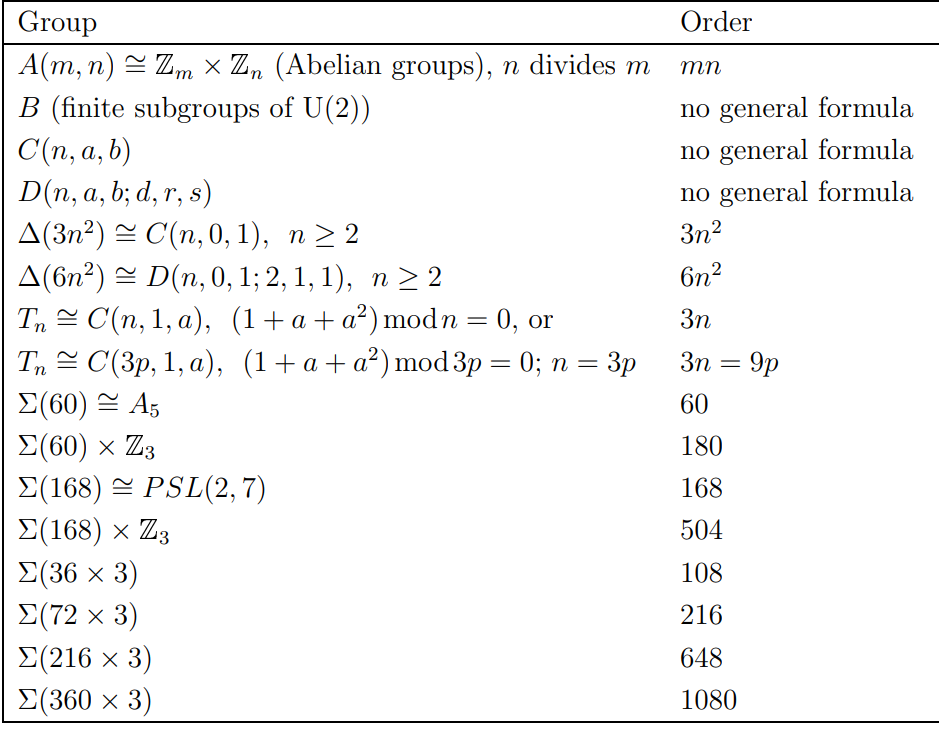
\includegraphics[scale=0.4]{img.png}
\end{figure}
Above is a table of all of the types of finite abelian subgroups that have been discovered. The only subgroup that I wish to discuss is the first one, as we are all familiar with the $\Z_m \times \Z_n$ groups\footnote{simple shorthand for $\Z/m\Z \times \Z/n\Z$}.
\begin{thm}
For all abelian subgroups A of $SU(3)$ is isomorphic to $\Z_m \times \Z_n$ such that $n|m$ and
\[ m = a' \]
we will denote $a'$ as the element $a \in A$ with the highest order.
\end{thm}
\begin{proof}
A is an abelian group of $3 \times 3$ matrices. Remember that for all $a \in A$ we need to make sure that $det(a) = 1$. Thus, if we are to create a basis for the group it would have to look like
\[
	\left[ \begin{matrix}
	a & 0 & 0\\
	0 & b & 0\\
	0 & 0 & a^{-1}b^{-1}
	\end{matrix} \right]
\]
such that $a,b \in U(1)$\\
This would then mean that $a^m = e$ where $e$ is the identity element. Suppose that for all $a \in A$ that $a^m \neq e$(m is not divisible by $|a|$). Let $g = gcd(|a|,m)$ and $g < |a|$. let $b$ be an element of $A$ such that $|b| = m$\\
This would then mean that $<a^g> \cap <b> = \{e\}$ for any $a,b \in A$, then
\[ |a^g \cdot b| = |a^g| \cdot |b| = \frac{|a|}{g} \cdot m > m\]
This leads to a contradiction to our earlier statement of $m = a'$.\\
From this, let $\mu = exp(2\pi i/m)$
\[
	\left[\begin{matrix}
	\mu^i & 0 & 0\\
	0 & \mu^j & 0\\
	0 & 0 & \mu^{-i-j}
	\end{matrix}\right]
\]
such that $0 \leq i,j \leq m-1$. We can then say that $A$ is a subgroup of:
\[
	\left\langle 
	\left[\begin{matrix}
	\mu & 0 & 0\\
	0 & 1 & 0\\
	0 & 0 & \mu^{-1}
	\end{matrix}\right],
	\left[\begin{matrix}
	1 & 0 & 0\\
	0 & \mu & 0\\
	0 & 0 & \mu^{-1}
	\end{matrix}\right] 	
	\right\rangle \cong \Z_m \times \Z_n
\]
Next we can treat m as a multiplicative sum of primes.
\[ m = p_1^{k_1} \times p_2^{k_2} \times ... \times p_i^{k_i} \]
\[ \Z_m = \Z_{p_1^{k_1}} \times \Z_{p_2^{k_2}} \times ... \times \Z_{p_i^{k_i}} \]
\[ \Z_m \times \Z_m = (\Z_{p_1^{k_1}} \times \Z_{p_1^{k_1}}) \times ... \times (\Z_{p_i^{k_i}} \times \Z_{p_i^{k_i}}) \]
\[ A \cong (\Z_{p_1^{r_1}} \times \Z_{p_1^{n_1}}) \times ... \times (\Z_{p_i^{r_i}} \times \Z_{p_i^{n_i}}) \cong \Z_r \times \Z_n \]
From out earlier proof by contradiction, we can then assume that r = m. Which shows that the isomorphism is true.\\
\end{proof}
%Bibliography
\section{SU(3) and the Standard Model}
\subsection{Introduction to the Standard Model}
The standard model is the current best model for particles. Essentially, it is the best theory we have as of right now that explains why things exist and how the universe's building blocks interact with each other. The particles within the standard model can be labeled into four different categories. There are two main categories which then split off into two separate ones of themselves. \\\\
There are the elementary fermions; this is then split into quarks and leptons. There are six different types of quarks: up, down, charm, strange, top, and bottom. Then there are also six different leptons: the electrons, muons, tau, and neutrino versions for each of the three leptons. Quarks are what make up most of the atoms in our world. For example, protons contain two up quarks, one down quark, and neutrons containing two down quarks and one up quark.\\\\
Next are the elementary bosons, which are split into gauge bosons and scalar bosons. Gauge bosons are responsible for the different types of forces that we have observed in the universe consisting of photons(electromagnetic), W, Z(weak force), and gluons(strong force). Finally, the only scalar boson is the Higgs boson; this particle is essentially responsible for giving things mass in the world.\\\\
There are a lot more details that I have left out as the standard model is quite vast. However, what I do want to focus on are the relationship between the quarks, gluons, and SU(3)

\subsection{SU(3) and gluons}
According to the standard model, the connection between quarks is due to gluons. Each quark supposedly carries a color charge, either red, green or blue. In order for the gluons to connect these quarks, the gluon has to carry an anti-charge. So anti-red, ant-green or anti-blue. Logically, if you were to pair regular color charges and anti charges, there would be 9 different types of gluons. However, the standard model states that there are only eight.\\\\
Let r,b,g be red blue and green respectively, and $\bar{r}, \bar{b}, \bar{g}$ be the anti versions of the colors
\begin{align*}
	r &= \left[ \begin{matrix}
	1\\ 0\\ 0
	\end{matrix} \right]
	b = \left[ \begin{matrix}
	0\\ 1\\ 0
	\end{matrix} \right]
	g = \left[ \begin{matrix}
	0\\ 0\\ 1
	\end{matrix} \right] \\
	\bar{r} &= \left[ \begin{matrix}
	1 & 0 & 0
	\end{matrix} \right]
	\bar{b} = \left[ \begin{matrix}
	0 & 1 & 0
	\end{matrix} \right]
	\bar{g} = \left[ \begin{matrix}
	0 & 0 & 1
	\end{matrix} \right]
\end{align*}
With this representation we can say that this $3 \times 3$ matrix is the red and anti-blue connection
\[
	\left[ \begin{matrix}
	0 & 1 & 0\\
	0 & 0 & 0\\
	0 & 0 & 0
	\end{matrix} \right]
\]
This is because the 1 is in the top row, and the middle column, so $r$ and $\bar{b}$\\
If we apply this logic to the eight generators of $SU(3)$ we will get the eight different types of gluons.
\[
\lambda_1 = \left[ \begin{matrix}
	0 & 1 & 0\\
	1 & 0 & 0\\
	0 & 0 & 0
	\end{matrix} \right] = (r\bar{b} + b\bar{r})/\sqrt{2}
\]\[
\lambda_2 = \left[ \begin{matrix}
	0 & -i & 0\\
	i & 0 & 0\\
	0 & 0 & 0
	\end{matrix} \right] = -i(r\bar{b} - b\bar{r})/\sqrt{2}
\]\[
\lambda_3 = \left[ \begin{matrix}
	1 & 0 & 0\\
	0 & -1 & 0\\
	0 & 0 & 0
	\end{matrix} \right] = (r\bar{r} - b\bar{b})/\sqrt{2}
\]\[
\lambda_4 = \left[ \begin{matrix}
	0 & 0 & 1\\
	0 & 0 & 0\\
	1 & 0 & 0
	\end{matrix} \right] = (r\bar{g} + g\bar{r})/\sqrt{2}
\]\[
\lambda_5 = \left[ \begin{matrix}
	0 & 0 & -i\\
	0 & 0 & 0\\
	1 & 0 & 0
	\end{matrix} \right] = -i(r\bar{g} - g\bar{r})/\sqrt{2}
\]\[
\lambda_6 = \left[ \begin{matrix}
	0 & 0 & 0\\
	0 & 0 & 1\\
	0 & 1 & 0
	\end{matrix} \right] = (b\bar{g} + g\bar{b})/\sqrt{2}
\]\[
\lambda_7 = \left[ \begin{matrix}
	0 & 0 & 0\\
	0 & 0 & -i\\
	0 & i & 0
	\end{matrix} \right] = -i(b\bar{g} - g\bar{b})/\sqrt{2}
\]\[
\lambda_8 = \frac{1}{\sqrt{3}}\left[ \begin{matrix}
	1 & 0 & 0\\
	0 & 1 & 0\\
	0 & 0 & -2
	\end{matrix} \right] = (r\bar{r} + b\bar{b} - 2g\bar{g})/\sqrt{6}
\]
You can see that in this representation that the matrices all have to be Hermitian and traceless. This makes the group $SU(3)$ a perfect representation of the gluon colors. There eight "colors" are known as the color octet and they represent the eight states that a gluon can be in. Every single one of these states are linearly independent from each other, which means that it is impossible to recreate any of them by combining others together.
%-------------------------------------------------------------------------------------------------------------------------------------------------------------------------------------
\newpage
\begin{thebibliography}{book}
\bibitem{ludlpatrick} Ludl, Patrick. Comments on the calssification of the finite subgroups of SU(3). {\it Journal of Algebra}. {\bf 114} (1988). pp. 115-259. 

\bibitem{ludlpatrick} Ludl, Patrick. Comments on the calssification of the finite subgroups of SU(3).(2011).

\bibitem{kiblermaurice} Kibler, Maurice. A Group-Theoretical Approach to the Periodic Table of Chemical Elements: Old and New Developments.

\bibitem{ludlpatrick} Kirillov, Alexander. Introduction to Lie Groups and Lie Algebras. 

\bibitem{ludlpatrick} Koerber, Christopher. Lie Algebra Tepresentation Theory-SU(3)-Representation in Physics.(2013) 

\bibitem{} “Why Are There Eight Gluons and Not Nine?” Why Are There Eight Gluons?, math.ucr.edu/home/baez/physics/ParticleAndNuclear/gluons.html. 
\end{thebibliography}


%-------------------------------------------------------------------------------------------------------------------------------------------------------------------------------------

%END

%-------------------------------------------------------------------------------------------------------------------------------------------------------------------------------------

\end{document} 